\documentclass[11pt]{article}
\usepackage{amsmath, amssymb, physics, mathtools, bm}
\usepackage{tikz, pgfplots}
\pgfplotsset{compat=1.18}
\usepackage[margin=2.3cm]{geometry}
\usepackage{siunitx, booktabs, hyperref}
\usepackage{braket}

\newcommand{\D}{\mathrm{D}}
\newcommand{\de}{\mathrm{d}}
\newcommand{\pd}[2]{\frac{\partial #1}{\partial #2}}
\newcommand{\pdd}[2]{\frac{\partial^{2} #1}{\partial #2^{2}}}
\newcommand{\Lap}{\nabla^{2}}

\title{B2 Symmetry and Relativity --- Model Solutions, 2017}
\author{}
\date{}

\begin{document}
\maketitle

%==================================================================
\section*{Question 1 --- 4-vectors, pure force, annihilation}

\textbf{Problem.} Define $\bm U$, $\bm F$; show orthogonal non-zero 4-vectors split into space-/time-like; show $\bm P\cdot\bm P=0\Rightarrow m=0$. Define proper time, pure force; show $\bm F\cdot\bm U=0$ and (with $\vb v\perp\vb a$) $A^\mu A_\mu=\gamma^4 a^2$. Solve constant pure-force motion; treat $e^+e^-$ annihilation; find $\gamma,\beta$ for an $e^-$ accelerated through $L=\SI{3}{m}$ in $E=\SI{10}{MV/m}$.

\subsection*{(a) Definitions and 4-orthogonality}

4-velocity and 4-force:
\[
U^\mu = \dv{X^\mu}{\tau} = \gamma(c,\vb v),\qquad F^\mu = \dv{P^\mu}{\tau},\quad P^\mu = m U^\mu.
\]

Orthogonality $\bm D\cdot\bm G=0$ with both non-zero. Assume $\bm D$ is time-like and boost to its rest frame:
\[
\bm D = (D^0,\vb 0),\qquad D^0\neq 0.
\]
Expand the inner product in this frame:
\[
\bm D\cdot\bm G = D^0 G^0 = 0.
\]
Divide by $D^0\neq 0$:
\[
G^0 = 0.
\]
Compute the invariant norm of $\bm G$:
\[
\bm G\cdot\bm G = (G^0)^2 - |\vb G|^2 = -|\vb G|^2.
\]
Use $\bm G\neq 0$ with $G^0=0$, so $\vb G\neq\vb 0$:
\[
\bm G\cdot\bm G < 0.
\]
Hence $\bm G$ is space-like whenever $\bm D$ is time-like. Symmetrically, if $\bm G$ is time-like then $\bm D$ is space-like. Two time-like vectors cannot be orthogonal: in the rest frame of one, the other still has non-zero time component (a time-like 4-vector has $G^0\neq 0$ in every frame), so $D^0 G^0\neq 0$. Therefore exactly one is time-like and the other space-like. \hfill$\square$

Invariant norm of 4-momentum:
\[
\bm P\cdot\bm P = \frac{E^2}{c^2} - |\vb p|^2 = m^2 c^2.
\]
Set $\bm P\cdot\bm P = 0$:
\[
m^2 c^2 = 0.
\]
Solve for $m$:
\[
\boxed{\,m=0\,}.
\]
Example: photon.

\subsection*{(b) Proper time, pure force, $A^\mu A_\mu=\gamma^4 a^2$}

\textbf{Proper time:} time interval recorded by a clock comoving with the particle, $\de\tau = \de t/\gamma$.
\textbf{Pure force:} a 4-force that does not change rest mass, $\dv*{m}{\tau}=0$.

Start from $\bm P\cdot\bm P = m^2 c^2$:
\[
P^\mu P_\mu = m^2 c^2.
\]
Differentiate w.r.t. $\tau$:
\[
2 P^\mu \dv{P_\mu}{\tau} = 2 m c^2 \dv{m}{\tau}.
\]
Identify $\dv*{P^\mu}{\tau}=F^\mu$:
\[
P^\mu F_\mu = m c^2 \dv{m}{\tau}.
\]
Pure force gives $\dv*{m}{\tau}=0$:
\[
P^\mu F_\mu = 0.
\]
Divide by $m$ using $P^\mu = m U^\mu$:
\[
\boxed{\;\bm F\cdot\bm U = 0\;}.
\]

4-acceleration: $A^\mu = \dv*{U^\mu}{\tau}$. Convert proper-time to lab-time via $\de\tau=\de t/\gamma$:
\[
A^\mu = \gamma\dv{t}\bigl(\gamma c,\gamma\vb v\bigr).
\]
Expand the derivative component by component:
\[
A^\mu = \bigl(\gamma\dot\gamma c,\;\gamma\dot\gamma\vb v + \gamma^2\vb a\bigr).
\]
Use the standard identity $\dot\gamma = \gamma^3(\vb v\cdot\vb a)/c^2$:
\[
\dot\gamma = \gamma^3(\vb v\cdot\vb a)/c^2.
\]
Apply $\vb v\perp\vb a$, so $\vb v\cdot\vb a = 0$:
\[
\dot\gamma = 0.
\]
Substitute back:
\[
A^\mu = (0,\gamma^2 \vb a).
\]
Square in $(+,-,-,-)$ signature:
\[
A^\mu A_\mu = (A^0)^2 - |\vb A|^2 = 0 - \gamma^4 a^2.
\]
Take the magnitude:
\[
\boxed{\;|A^\mu A_\mu| = \gamma^4 a^2\;}.
\]

\subsection*{(c) Constant pure force on rest mass $M_0$}

Newton's law in lab time with constant 3-force $f_x$:
\[
\dv{p_x}{t} = f_x.
\]
Integrate with initial condition $p_x(0)=0$:
\[
p_x(t) = f_x t.
\]
Energy--momentum relation:
\[
E^2 = (M_0 c^2)^2 + (p_x c)^2.
\]
Substitute $p_x = f_x t$:
\[
E(t)^2 = (M_0 c^2)^2 + (f_x t c)^2.
\]
Take the square root:
\[
E(t) = c\sqrt{(M_0 c)^2 + (f_x t)^2}.
\]
Use $U^0 = E/(M_0 c)$:
\[
U^0 = \frac{c\sqrt{(M_0 c)^2 + (f_x t)^2}}{M_0 c}.
\]
Factor $M_0 c$ inside the root:
\[
U^0 = c\sqrt{1+\bigl(f_x t/(M_0 c)\bigr)^2}.
\]
Use $U^1 = p_x/M_0$:
\[
U^1 = \frac{f_x t}{M_0}.
\]
Assemble $U^\mu$:
\[
\boxed{\;U^\mu = \biggl(c\sqrt{1 + (f_x t/(M_0 c))^2},\;\frac{f_x t}{M_0},\;0,\;0\biggr)\;}.
\]
Read off $\gamma = U^0/c$:
\[
\gamma(t) = \sqrt{1 + \bigl(f_x t/(M_0 c)\bigr)^2}.
\]
Use $\beta = p_x c/E$:
\[
\beta(t) = \frac{f_x t}{\sqrt{(M_0 c)^2 + (f_x t)^2}}.
\]
Limits: $\beta(0)=0$, $\gamma(0)=1$; $\beta\to 1$ and $\gamma\to f_x t/(M_0 c)$ as $t\to\infty$.

\begin{center}
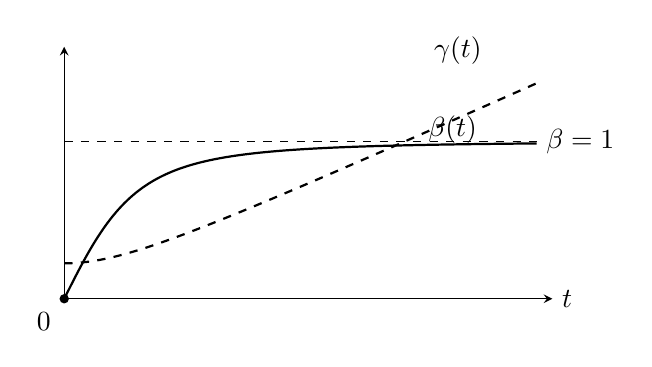
\begin{tikzpicture}[>=stealth, scale=1.0]
  \draw[->] (0,0) -- (6.2,0) node[right] {$t$};
  \draw[->] (0,0) -- (0,3.2) node[above] {};
  \draw[dashed] (0,2) -- (6,2) node[right] {$\beta=1$};
  \draw[thick, domain=0:6, samples=80, smooth] plot (\x, {2*\x/sqrt(1+\x*\x)});
  \node[above right] at (4.5,1.85) {$\beta(t)$};
  \draw[thick, dashed, domain=0:6, samples=80, smooth] plot (\x, {sqrt(1+\x*\x)*0.45});
  \node[above] at (5.0,2.85) {$\gamma(t)$};
  \node[circle,fill,inner sep=1.2pt,label=below left:{$0$}] at (0,0) {};
\end{tikzpicture}
\end{center}

\subsection*{(d) $e^+e^-$ annihilation at rest --- minimum photon count}

Initial system has zero net 3-momentum (head-on, equal speeds, equal mass). A single photon would carry $|\vb p|=E_\gamma/c\neq 0$, violating momentum conservation. Hence
\[
\boxed{\;N_{\min}=2\;}\quad\text{(back-to-back, equal energy)}.
\]
Energy conservation in lab frame:
\[
2 E_\gamma = (T_{e^-} + m_e c^2) + (T_{e^+} + m_e c^2).
\]
Group kinetic and rest-energy terms:
\[
2 E_\gamma = T_\text{tot} + 2 m_e c^2.
\]
Substitute $T_\text{tot}=1000$ MeV, $m_e c^2 = 0.511$ MeV:
\[
2 E_\gamma = 1000 + 2(0.511).
\]
Evaluate the right-hand side:
\[
2 E_\gamma = 1001.022\;\text{MeV}.
\]
Divide by 2:
\[
\boxed{\;E_\gamma \approx 500.5\;\text{MeV}\;}.
\]

\subsection*{(e) Electron through $L=\SI{3}{m}$ at $E=\SI{10}{MV/m}$}

Kinetic energy gained equals work done by the field:
\[
T = eEL.
\]
Substitute $eE=\SI{10}{MeV/m}$, $L=\SI{3}{m}$:
\[
T = (10\;\text{MeV/m})\times(3\;\text{m}).
\]
Evaluate:
\[
T = 30\;\text{MeV}.
\]
Compute total energy $W = T + m_e c^2$:
\[
W = 30 + 0.511\;\text{MeV} = 30.511\;\text{MeV}.
\]
Lorentz factor $\gamma = W/(m_e c^2)$:
\[
\gamma = \frac{30.511}{0.511}.
\]
Evaluate:
\[
\boxed{\;\gamma \approx 59.7\;}.
\]
Compute $1/\gamma^2$:
\[
1/\gamma^2 \approx 2.81\times 10^{-4}.
\]
Apply $\beta = \sqrt{1 - 1/\gamma^2}$:
\[
\beta = \sqrt{1 - 2.81\times 10^{-4}}.
\]
Evaluate:
\[
\boxed{\;\beta \approx 0.99986\;}.
\]

%==================================================================
\section*{Question 2 --- 4-wavevector, simultaneity, fields, photon-gas invariant}

\textbf{Problem.} Components of $\bm K$; phase invariance; isolated electron cannot emit a photon; space-like condition and simultaneity frame; two-photon system invariant mass and CoM velocity; non-relativistic motion in crossed $\vb E,\vb B$ for $|E/B|\gtrless c$; invariance of $s^2=(\sum W)^2-|\sum\vb p|^2$ and its value for a photon gas.

\subsection*{(a) 4-wavevector, phase invariance, no spontaneous photon emission}

For a plane EM wave $\psi\propto e^{i(\vb k\cdot\vb x-\omega t)}$ in vacuum with $|\vb k|=\omega/c$:
\[
K^\mu = (\omega/c,\,\vb k).
\]
Form the contraction $K_\mu X^\mu$ with $X^\mu=(ct,\vb x)$:
\[
K_\mu X^\mu = (\omega/c)(ct) - \vb k\cdot\vb x = \omega t - \vb k\cdot\vb x.
\]
Identify the wave phase:
\[
\varphi = \vb k\cdot\vb x - \omega t = -K_\mu X^\mu.
\]
Contraction of two 4-vectors is a Lorentz scalar:
\[
\boxed{\;\varphi'=\varphi\;}.
\]

Hypothetical process $e^-\to e^- + \gamma$ in vacuum. Work in the initial electron rest frame:
\[
\bm P_e = (m_e c,\vb 0).
\]
4-momentum conservation:
\[
\bm P_e = \bm P_e' + \hbar\bm K_\gamma.
\]
Read off 3-momentum: $\vb p_e' = -\hbar\vb k_\gamma$:
\[
|\vb p_e'| = \hbar|\vb k_\gamma| = \hbar\omega/c.
\]
Apply energy-momentum relation to the final electron:
\[
E_e' = \sqrt{(m_e c^2)^2+|\vb p_e'|^2 c^2} = \sqrt{(m_e c^2)^2+(\hbar\omega)^2}.
\]
Apply energy conservation:
\[
m_e c^2 = \sqrt{(m_e c^2)^2+(\hbar\omega)^2} + \hbar\omega.
\]
Isolate the square root:
\[
m_e c^2 - \hbar\omega = \sqrt{(m_e c^2)^2+(\hbar\omega)^2}.
\]
Square both sides:
\[
(m_e c^2)^2 - 2 m_e c^2\hbar\omega + (\hbar\omega)^2 = (m_e c^2)^2 + (\hbar\omega)^2.
\]
Cancel $(m_e c^2)^2$ and $(\hbar\omega)^2$:
\[
-2 m_e c^2 \hbar\omega = 0.
\]
Solve for $\omega$:
\[
\omega = 0.
\]
No physical photon emission possible. \hfill$\square$

\subsection*{(b) Space-like interval, simultaneity}

Invariant interval between $\bm D$ and $\bm G$:
\[
(\bm D-\bm G)\cdot(\bm D-\bm G) = c^2(t_d-t_g)^2 - |\vb x_d-\vb x_g|^2.
\]
Space-like condition (interval $<0$):
\[
\boxed{\;|\vb x_d-\vb x_g|^2 > c^2(t_d-t_g)^2\;}.
\]
Boost with velocity $\vb V$ parallel to $\Delta\vb x = \vb x_d-\vb x_g$:
\[
\Delta t' = \gamma_V\bigl(\Delta t - \vb V\cdot\Delta\vb x/c^2\bigr).
\]
Set $\Delta t'=0$ (simultaneity in $S'$):
\[
\Delta t = \vb V\cdot\Delta\vb x/c^2.
\]
Use $\vb V\parallel\Delta\vb x$, so $\vb V\cdot\Delta\vb x = V|\Delta\vb x|$:
\[
V = \frac{c^2\,\Delta t}{|\Delta\vb x|}.
\]
Compute $|V|/c$:
\[
|V|/c = \frac{c|\Delta t|}{|\Delta\vb x|}.
\]
Apply the space-like condition $c|\Delta t|<|\Delta\vb x|$:
\[
|V|/c < 1.
\]
Hence a real boost exists --- such a frame $S'$ exists.

\subsection*{(c) Two perpendicular photons of equal $\omega$}

4-momenta of two photons (components $(E/c,\vb p)$) with $|\vb p|=\hbar\omega/c$:
\[
\bm P_1 = \frac{\hbar\omega}{c}(1,1,0,0),\qquad \bm P_2 = \frac{\hbar\omega}{c}(1,0,1,0).
\]
Add the 4-momenta:
\[
\bm P = \bm P_1+\bm P_2 = \frac{\hbar\omega}{c}(2,1,1,0).
\]
Form the invariant norm in $(+,-,-,-)$:
\[
\bm P\cdot\bm P = \biggl(\frac{\hbar\omega}{c}\biggr)^2\bigl(2^2 - 1^2 - 1^2\bigr).
\]
Evaluate:
\[
\bm P\cdot\bm P = 2\biggl(\frac{\hbar\omega}{c}\biggr)^2.
\]
Identify $\bm P\cdot\bm P = M^2 c^2$:
\[
M^2 c^2 = 2\biggl(\frac{\hbar\omega}{c}\biggr)^2.
\]
Solve for $M$:
\[
\boxed{\;M = \frac{\sqrt{2}\,\hbar\omega}{c^2}\;}.
\]
CoM velocity formula: $\vb v_\text{CoM} = c^2\vb p_\text{tot}/E_\text{tot}$. Read off totals:
\[
\vb p_\text{tot} = \frac{\hbar\omega}{c}(1,1,0),\qquad E_\text{tot} = 2\hbar\omega.
\]
Substitute:
\[
\vb v_\text{CoM} = \frac{c^2(\hbar\omega/c)(1,1,0)}{2\hbar\omega}.
\]
Cancel $\hbar\omega$:
\[
\vb v_\text{CoM} = \frac{c}{2}(1,1,0).
\]
Compute the magnitude:
\[
|\vb v_\text{CoM}| = \frac{c}{2}\sqrt{1^2+1^2} = \frac{c}{\sqrt 2}.
\]
Final answer:
\[
\boxed{\;\vb v_\text{CoM} = (c/2,\,c/2,\,0),\quad|\vb v_\text{CoM}|=c/\sqrt{2}\;}.
\]

\subsection*{(d) Electron in crossed $\vb E\perp\vb B$}

Field invariants:
\[
\vb E\cdot\vb B = 0,\qquad I_2 = E^2 - c^2 B^2.
\]
Compute $\vb E\times\vb B$ with $\vb E=(0,E,0),\;\vb B=(0,0,B)$:
\[
\vb E\times\vb B = E\hat{\vb y}\times B\hat{\vb z} = EB\hat{\vb x}.
\]

\textbf{Case (a): $|E/B|>c$, so $I_2 > 0$.} Choose boost along $\hat{\vb x}$ that eliminates $\vb B'$:
\[
\vb v_d = \frac{c^2\,\vb E\times\vb B}{E^2} = \biggl(\frac{c^2 B}{E},0,0\biggr).
\]
Check $|\vb v_d|/c < 1$:
\[
|\vb v_d|/c = cB/E < 1\quad(\text{since }E/B>c).
\]
Define $\gamma_d = 1/\sqrt{1-c^2 B^2/E^2}$. Compute $E_y'$:
\[
E_y' = \gamma_d(E_y - v_d B_z) = \gamma_d\bigl(E - (c^2 B/E)\,B\bigr).
\]
Factor $E$:
\[
E_y' = \gamma_d E\bigl(1 - c^2 B^2/E^2\bigr).
\]
Use $1 - c^2 B^2/E^2 = 1/\gamma_d^2$:
\[
E_y' = E/\gamma_d.
\]
Compute $B_z'$:
\[
B_z' = \gamma_d(B_z - v_d E_y/c^2) = \gamma_d\bigl(B - (c^2 B/E)(E)/c^2\bigr).
\]
Cancel inside the bracket:
\[
B_z' = 0.
\]
Hence $\vb B'=0$ and $\vb E'=(E/\gamma_d)\hat{\vb y}$. Equation of motion in $S'$ for electron of charge $-e$:
\[
\dv{\vb p'}{t'} = -e\vb E'.
\]
Initial condition: electron at rest in $S$, so in $S'$ it moves at $-\vb v_d\hat{\vb x}'$. Result: uniform acceleration along $-\hat{\vb y}'$ superposed on $-\vb v_d\hat{\vb x}'$, giving relativistic hyperbolic motion in $S'$ (no closed orbit).
In lab frame $S$: add drift $+\vb v_d\hat{\vb x}$ — particle is continuously accelerated and drifts in $+\hat{\vb x}$, an open unbounded trajectory.

\textbf{Case (b): $|E/B|<c$, so $I_2 < 0$.} Choose boost along $\hat{\vb x}$ that eliminates $\vb E'$:
\[
\vb v_d = \frac{\vb E\times\vb B}{B^2} = \biggl(\frac{E}{B},0,0\biggr),\quad|\vb v_d|<c.
\]
Define $\gamma_d = 1/\sqrt{1-E^2/(c^2 B^2)}$. Compute $E_y'$:
\[
E_y' = \gamma_d(E_y - v_d B_z) = \gamma_d\bigl(E - (E/B)B\bigr).
\]
Cancel inside the bracket:
\[
E_y' = 0.
\]
Compute $B_z'$:
\[
B_z' = \gamma_d(B_z - v_d E_y/c^2) = \gamma_d B\bigl(1 - E^2/(c^2 B^2)\bigr).
\]
Use $1 - E^2/(c^2 B^2) = 1/\gamma_d^2$:
\[
B_z' = B/\gamma_d.
\]
Hence $\vb E'=0$ and $\vb B'=(B/\gamma_d)\hat{\vb z}$. Equation of motion in $S'$:
\[
\dv{\vb p'}{t'} = -e\,\vb v'\times\vb B'.
\]
Initial condition: in $S'$ electron moves at $-\vb v_d\hat{\vb x}'$. Pure magnetic field gives a closed circular orbit in the $x'y'$-plane of radius $r' = p'/(eB')$.
In lab frame $S$: add drift $+\vb v_d\hat{\vb x}$ — cycloid drifting along $+\hat{\vb x}$ at speed $E/B$.

\begin{center}
\begin{tikzpicture}[>=stealth, scale=0.85]
  % Case (a)
  \begin{scope}[xshift=-4.5cm]
  \draw[->] (-0.2,0) -- (5.0,0) node[right] {$x$};
  \draw[->] (0,-0.2) -- (0,3.0) node[above] {$y$};
  \draw[thick, domain=0:4.5, samples=60, smooth] plot (\x, {0.25*\x*\x});
  \node[circle,fill,inner sep=1.2pt,label=below left:{$0$}] at (0,0) {};
  \node[above] at (2.5,-1.2) {Case (a): $|E/B|>c$};
  \end{scope}
  % Case (b)
  \begin{scope}[xshift=4.0cm]
  \draw[->] (-0.2,0) -- (5.5,0) node[right] {$x$};
  \draw[->] (0,-0.2) -- (0,3.0) node[above] {$y$};
  \draw[thick, domain=0:4.5*pi/2, samples=120, smooth]
        plot ({\x/2 - 0.5*sin(2*\x r)}, {0.5 - 0.5*cos(2*\x r)});
  \node[circle,fill,inner sep=1.2pt,label=below left:{$0$}] at (0,0) {};
  \node[above] at (2.5,-1.2) {Case (b): $|E/B|<c$ (cycloid)};
  \end{scope}
\end{tikzpicture}
\end{center}

\subsection*{(e) Invariance of $s^2$ for non-interacting system}

Define total 4-momentum:
\[
\bm P_\text{tot} = \sum_i \bm P_i.
\]
Sum of 4-vectors is a 4-vector; non-interacting particles have each $\bm P_i$ conserved.
Form the invariant norm (with $c=1$):
\[
\bm P_\text{tot}\cdot\bm P_\text{tot} = \biggl(\sum_i W_i\biggr)^2 - \biggl|\sum_i\vb p_i\biggr|^2 = s^2.
\]
Inner product of a 4-vector with itself is a Lorentz scalar, so $s^2$ is invariant. \hfill$\square$

Photon gas: each photon satisfies $\bm P_i\cdot\bm P_i = W_i^2 - |\vb p_i|^2 = 0$, so $|\vb p_i|=W_i$. Expand the squared norm:
\[
s^2 = \sum_i \bm P_i\cdot\bm P_i + 2\sum_{i<j}\bm P_i\cdot\bm P_j.
\]
Drop the null self-terms:
\[
s^2 = 2\sum_{i<j}\bm P_i\cdot\bm P_j.
\]
Expand each inner product:
\[
\bm P_i\cdot\bm P_j = W_i W_j - \vb p_i\cdot\vb p_j.
\]
Substitute $\vb p_i\cdot\vb p_j = |\vb p_i||\vb p_j|\cos\theta_{ij} = W_i W_j\cos\theta_{ij}$:
\[
\bm P_i\cdot\bm P_j = W_i W_j(1-\cos\theta_{ij}).
\]
Sum over pairs:
\[
\boxed{\;s^2 = 2\sum_{i<j} W_i W_j(1-\cos\theta_{ij})\;\geq 0\;}.
\]

%==================================================================
\section*{Question 3 --- Astrophysical SR tests, Doppler, elastic collision, undulator}

\textbf{Problem.} Three astrophysical SR tests; Compton shift; relativistic Doppler longitudinal and transverse; equal-mass elastic-collision angle theorem; field of a static undulator in the electron rest frame.

\subsection*{(a) Three astrophysical tests; Compton shift}

Three direct SR tests via emitted/reflected light:
\begin{enumerate}
\item Cosmological redshift of distant galaxies (relativistic Doppler).
\item Time dilation of supernova light curves (Type-Ia at high $z$).
\item Aberration of starlight / transverse Doppler from rapidly moving stellar systems (or relativistic beaming in jets).
\end{enumerate}

Compton scattering: incoming photon $\hbar\bm K=(\hbar\omega/c,\hbar\vb k)$, electron at rest $\bm P_e=(m_e c,\vb 0)$. Outgoing: photon $\hbar\bm K'=(\hbar\omega'/c,\hbar\vb k')$, electron $\bm P_e'$ with $\bm P_e'\cdot\bm P_e' = m_e^2c^2$.

Apply 4-momentum conservation:
\[
\hbar\bm K + \bm P_e = \hbar\bm K' + \bm P_e'.
\]
Isolate the scattered electron:
\[
\bm P_e' = \hbar\bm K - \hbar\bm K' + \bm P_e.
\]
Square both sides (take invariant norm):
\[
\bm P_e'\cdot\bm P_e' = \bigl(\hbar\bm K - \hbar\bm K' + \bm P_e\bigr)\cdot\bigl(\hbar\bm K - \hbar\bm K' + \bm P_e\bigr).
\]
Expand the right-hand side:
\[
m_e^2 c^2 = \hbar^2\bm K\cdot\bm K + \hbar^2\bm K'\cdot\bm K' - 2\hbar^2\bm K\cdot\bm K' + 2\hbar\bm P_e\cdot\bm K - 2\hbar\bm P_e\cdot\bm K' + m_e^2 c^2.
\]
Apply $\bm K\cdot\bm K=\bm K'\cdot\bm K'=0$ (massless photons):
\[
0 = -2\hbar^2\bm K\cdot\bm K' + 2\hbar\bm P_e\cdot\bm K - 2\hbar\bm P_e\cdot\bm K'.
\]
Divide by $2\hbar$:
\[
\bm P_e\cdot\bm K - \bm P_e\cdot\bm K' = \hbar\bm K\cdot\bm K'.
\]
Compute $\bm P_e\cdot\bm K$ with $\bm P_e=(m_ec,\vb 0)$:
\[
\bm P_e\cdot\bm K = (m_e c)(\omega/c) - \vb 0\cdot\hbar\vb k = m_e\omega.
\]
Similarly:
\[
\bm P_e\cdot\bm K' = m_e\omega'.
\]
Compute $\bm K\cdot\bm K'$ with $|\vb k|=\omega/c$, $|\vb k'|=\omega'/c$:
\[
\bm K\cdot\bm K' = \frac{\omega\omega'}{c^2} - \vb k\cdot\vb k'.
\]
Substitute $\vb k\cdot\vb k' = (\omega\omega'/c^2)\cos\theta$:
\[
\bm K\cdot\bm K' = \frac{\omega\omega'}{c^2}(1-\cos\theta).
\]
Substitute into $\bm P_e\cdot\bm K - \bm P_e\cdot\bm K' = \hbar\bm K\cdot\bm K'$:
\[
m_e(\omega - \omega') = \frac{\hbar\omega\omega'}{c^2}(1-\cos\theta).
\]
Divide by $m_e\omega\omega'$:
\[
\frac{1}{\omega'} - \frac{1}{\omega} = \frac{\hbar}{m_e c^2}(1-\cos\theta).
\]
Final Compton formula:
\[
\boxed{\;\frac{1}{\omega'} - \frac{1}{\omega} = \frac{\hbar}{m_e c^2}(1-\cos\theta)\;}\;\Longleftrightarrow\;\Delta\lambda = \frac{h}{m_e c}(1-\cos\theta).
\]

\subsection*{(b) Doppler effect}

Phase $\varphi = -K_\mu X^\mu$ is Lorentz invariant; equivalently $\bm K$ transforms as a 4-vector. Vacuum dispersion gives $|\vb k|=\omega/c$, so with $\vb k=k_x\hat{\vb x}$:
\[
\bm K = (\omega/c,\omega/c,0,0).
\]

\textbf{Case (a): $\vb v=(v_x,0,0)$ parallel to $\vb k$ (longitudinal).}
Apply Lorentz boost along $\hat{\vb x}$ to $K^0$:
\[
K'^0 = \gamma(K^0 - \beta K^1).
\]
Substitute $K^0 = K^1 = \omega/c$:
\[
\omega'/c = \gamma(\omega/c - \beta\omega/c).
\]
Factor $\omega/c$:
\[
\omega' = \gamma\omega(1-\beta).
\]
Use $\gamma = 1/\sqrt{(1-\beta)(1+\beta)}$:
\[
\omega' = \omega\frac{1-\beta}{\sqrt{(1-\beta)(1+\beta)}}.
\]
Simplify the fraction:
\[
\boxed{\;\omega' = \omega\sqrt{\frac{1-\beta}{1+\beta}}\;}\quad(\text{longitudinal Doppler}).
\]

\textbf{Case (b): $\vb v=(0,v_y,0)$ perpendicular to $\vb k$ (transverse).}
Apply Lorentz boost along $\hat{\vb y}$ to $K^0$:
\[
K'^0 = \gamma(K^0 - \beta K^2).
\]
Substitute $K^2 = 0$:
\[
\omega'/c = \gamma\omega/c.
\]
Multiply by $c$:
\[
\boxed{\;\omega' = \gamma\omega\;}\quad(\text{transverse Doppler}).
\]

\subsection*{(c) Elastic collision: equal post-collision angles $\Rightarrow$ $M_1=M_2$}

Work in the CoM frame. By definition, total 3-momentum vanishes, so outgoing particles are back-to-back with equal momentum magnitude:
\[
|\vb p_1^*| = |\vb p_2^*| \equiv p^*.
\]
In elastic scattering CoM energies are conserved and fixed by the masses:
\[
E_i^* = \sqrt{p^{*2}c^2 + M_i^2 c^4}\quad(i=1,2).
\]
Let particle 1 emerge at angle $\phi^*$ above $+\hat{\vb x}$ in CoM; particle 2 at angle $\pi+\phi^*$:
\[
p^*_{1x}=p^*\cos\phi^*,\;p^*_{1y}=p^*\sin\phi^*;\quad p^*_{2x}=-p^*\cos\phi^*,\;p^*_{2y}=-p^*\sin\phi^*.
\]
Boost back to lab along $+\beta_\text{CoM}\hat{\vb x}$. Transverse momenta unchanged:
\[
p_{1y}^{\rm lab} = p^*\sin\phi^*,\qquad p_{2y}^{\rm lab} = -p^*\sin\phi^*.
\]
Transform longitudinal components:
\[
p_{1x}^{\rm lab} = \gamma_\text{CoM}\bigl(p^*\cos\phi^* + \beta_\text{CoM} E_1^*/c\bigr),
\]
\[
p_{2x}^{\rm lab} = \gamma_\text{CoM}\bigl(-p^*\cos\phi^* + \beta_\text{CoM} E_2^*/c\bigr).
\]
Define lab angles $\theta_i$ (above/below $\hat{\vb x}$) by $\tan\theta_i = |p_{iy}^{\rm lab}|/p_{ix}^{\rm lab}$:
\[
\tan\theta_1 = \frac{p^*\sin\phi^*}{\gamma_\text{CoM}(p^*\cos\phi^* + \beta_\text{CoM} E_1^*/c)},
\]
\[
\tan\theta_2 = \frac{p^*\sin\phi^*}{\gamma_\text{CoM}(-p^*\cos\phi^* + \beta_\text{CoM} E_2^*/c)}.
\]
Impose $\theta_1 = \theta_2$ (numerators equal, so denominators must be equal):
\[
p^*\cos\phi^* + \beta_\text{CoM} E_1^*/c = -p^*\cos\phi^* + \beta_\text{CoM} E_2^*/c.
\]
Rearrange:
\[
2p^*\cos\phi^* = \beta_\text{CoM}(E_2^* - E_1^*)/c.
\]
The CoM scattering angle $\phi^*$ depends on impact parameter and can take any value in $[0,\pi]$, while $E_1^*$, $E_2^*$, $p^*$, $\beta_\text{CoM}$ are fixed by initial kinematics. For $\theta_1=\theta_2$ to hold for the elastic scattering (independently of the impact parameter, i.e., for all $\phi^*$), the right-hand side must be independent of $\phi^*$ and equal the variable left-hand side; both sides must therefore vanish:
\[
E_1^* = E_2^* \quad\text{and}\quad \cos\phi^* = 0.
\]
Apply $|\vb p_1^*|=|\vb p_2^*|=p^*$ and the energy--momentum relation $E_i^{*2} - p^{*2}c^2 = M_i^2 c^4$:
\[
M_1^2 c^4 = (E_1^*)^2 - p^{*2}c^2 = (E_2^*)^2 - p^{*2}c^2 = M_2^2 c^4.
\]
Take the positive square root:
\[
\boxed{\;M_1 = M_2\;}.\qquad\square
\]

\subsection*{(d) Static undulator field in electron rest frame}

Lab potentials: $\vb A=(0,A_0\cos(k_u z),0)$, $\phi=0$. Compute the lab electric field:
\[
\vb E = -\partial_t \vb A - \nabla\phi = \vb 0.
\]
Compute the lab magnetic field $\vb B = \nabla\times\vb A$:
\[
B_x = \partial_y A_z - \partial_z A_y = -\partial_z[A_0\cos(k_u z)].
\]
Differentiate:
\[
B_x = A_0 k_u\sin(k_u z).
\]
Other components vanish:
\[
\vb B = A_0 k_u\sin(k_u z)\,\hat{\vb x}.
\]

Boost to electron rest frame along $+\hat{\vb z}$ with velocity $v\hat{\vb z}$, $\gamma=1/\sqrt{1-v^2/c^2}$. Apply field transformation $\vb E_\perp' = \gamma(\vb E_\perp + \vb v\times\vb B)$ with $\vb E=\vb 0$:
\[
\vb v\times\vb B = v\hat{\vb z}\times B_x\hat{\vb x} = v B_x\,\hat{\vb y}.
\]
Read off $E_y'$:
\[
E_y' = \gamma v B_x = \gamma v A_0 k_u \sin(k_u z).
\]
Other electric components:
\[
E_x' = 0,\qquad E_z' = E_z = 0.
\]
Apply magnetic transformation $\vb B_\perp' = \gamma(\vb B_\perp - \vb v\times\vb E/c^2)$ with $\vb E=0$:
\[
B_x' = \gamma B_x = \gamma A_0 k_u\sin(k_u z).
\]
Other magnetic components:
\[
B_y' = 0,\qquad B_z' = B_z = 0.
\]
Express $z$ in primed coordinates via inverse Lorentz transformation $z = \gamma(z' + v t')$:
\[
\boxed{\;\vb E' = \gamma v A_0 k_u \sin\!\bigl(k_u\gamma(z'+vt')\bigr)\,\hat{\vb y},\quad \vb B' = \gamma A_0 k_u \sin\!\bigl(k_u\gamma(z'+vt')\bigr)\,\hat{\vb x}\;}.
\]

Wave-like check. Compute ratio $|E'|/|B'|$:
\[
|E'|/|B'| = v.
\]
Read off wave-vector and frequency from the phase $k_u\gamma(z'+vt')$:
\[
k' = \gamma k_u,\qquad \omega' = \gamma v k_u.
\]
Compute phase velocity:
\[
\omega'/k' = v < c.
\]
Strictly $\omega'/k' \neq c$, so it is \emph{not} a vacuum EM wave; it is the Lorentz-transformed near-field of a static magnet. In the ultra-relativistic limit $v\to c$ it becomes indistinguishable from a propagating EM wave (basis of free-electron-laser/undulator radiation).

%==================================================================
\section*{Question 4 --- Field transformations, EM tensor, wires, inverse Compton}

\textbf{Problem.} Field transformations under boost along $x$; field tensor from a plane-wave 4-potential; Maxwell in covariant form; physical meaning of $f_0$; orthogonality of $U_W^\mu$ and $\bm P$; fields of a current-carrying wire in three frames and whether two wires can interact purely electrically; ultra-relativistic inverse Compton maximum.

\subsection*{(a) Field transformations, boost along $\hat{\vb x}$ with $\vb v=(v_x,0,0)$}

\[
\boxed{\;
\begin{aligned}
&E_x' = E_x,\quad E_y' = \gamma(E_y - v_x B_z),\quad E_z' = \gamma(E_z + v_x B_y),\\
&B_x' = B_x,\quad B_y' = \gamma(B_y + v_x E_z/c^2),\quad B_z' = \gamma(B_z - v_x E_y/c^2).
\end{aligned}
\;}
\]

\subsection*{(b) Field tensor from $\bm A$, Maxwell covariant form}

Definitions: 4-potential $\bm A = (\phi/c,\vb A)$ and 4-wave vector $\bm K=(\omega/c,\vb k)$.

For propagation along $\hat{\vb z}$ with $K^\mu = (\omega/c,0,0,k)$. Compute the phase $K^\mu X_\mu$ in $(+,-,-,-)$:
\[
K^\mu X_\mu = (\omega/c)(ct) - kz = \omega t - kz.
\]
Substitute into $A_y$:
\[
A_y = -\frac{\sin(\omega t - kz)}{\sqrt{\omega k}}.
\]
Differentiate w.r.t.\ $t$:
\[
\partial_t A_y = -\frac{\omega\cos(\omega t-kz)}{\sqrt{\omega k}}.
\]
Differentiate w.r.t.\ $z$:
\[
\partial_z A_y = \frac{k\cos(\omega t-kz)}{\sqrt{\omega k}}.
\]
Read off $E_y$ from $\vb E = -\partial_t\vb A - \nabla\phi$:
\[
E_y = -\partial_t A_y = \frac{\omega\cos(\omega t-kz)}{\sqrt{\omega k}} = \sqrt{\omega/k}\cos(\omega t-kz).
\]
Read off $B_x$ from $\vb B = \nabla\times\vb A$ (only $A_y$ non-zero, $A_y$ depends on $z,t$):
\[
B_x = -\partial_z A_y = -\sqrt{k/\omega}\cos(\omega t-kz).
\]
Compute $F^{02} = \partial^0 A^2 - \partial^2 A^0$ with $\partial^0=(1/c)\partial_t$, $A^0=0$, $A^2 = A_y$:
\[
F^{02} = (1/c)\partial_t A_y.
\]
Substitute $\partial_t A_y = -E_y$:
\[
F^{02} = -E_y/c.
\]
Compute $F^{32} = \partial^3 A^2 - \partial^2 A^3$ with $\partial^3=-\partial_z$, $A^3=0$:
\[
F^{32} = -\partial_z A_y = B_x.
\]
Field-tensor entries (independent non-zero ones, others fixed by antisymmetry):
\[
\boxed{\;F^{02} = -E_y/c,\;F^{32}=B_x;\quad E_y = \sqrt{\omega/k}\cos(\omega t-kz),\;B_x = -\sqrt{k/\omega}\cos(\omega t-kz)\;}.
\]

\textbf{4-current and continuity.} Define $J^\nu = (\rho c,\vb j)$. 3-vector continuity:
\[
\partial_t\rho + \nabla\cdot\vb j = 0.
\]
4-vector form:
\[
\boxed{\;\partial_\nu J^\nu = 0\;}.
\]

\textbf{Maxwell covariant form.} Compute $\partial_\mu F^{\mu 0}$ using $F^{00}=0$ and $F^{i0} = E^i/c$:
\[
\partial_\mu F^{\mu 0} = \partial_i F^{i0} = \nabla\cdot\vb E/c.
\]
Apply Gauss's law $\nabla\cdot\vb E = \rho/\epsilon_0$:
\[
\partial_\mu F^{\mu 0} = \rho/(c\epsilon_0).
\]
Use $\mu_0\epsilon_0 = 1/c^2$, i.e.\ $1/(c\epsilon_0)=\mu_0 c$:
\[
\partial_\mu F^{\mu 0} = \mu_0 c\rho = \mu_0 J^0.
\]
Compute $\partial_\mu F^{\mu i}$ using $F^{0i}=-E^i/c$ and $F^{ji}=-\epsilon^{jik}B_k$:
\[
\partial_\mu F^{\mu i} = (1/c)\partial_t(-E^i/c) + (\nabla\times\vb B)^i = -\partial_t E^i/c^2 + (\nabla\times\vb B)^i.
\]
Apply Amp\`ere--Maxwell $\nabla\times\vb B - (1/c^2)\partial_t\vb E = \mu_0\vb j$:
\[
\partial_\mu F^{\mu i} = \mu_0 j^i = \mu_0 J^i.
\]
Combine both cases:
\[
\boxed{\;\partial_\mu F^{\mu\nu} = \mu_0 J^\nu\;}.
\]

\textbf{Physical meaning of $f_0 = J^\nu F_{\nu 0}$.} Use $F_{00}=0$ and $F_{i0} = -F^{i0} = -E_i/c$:
\[
f_0 = J^0 F_{00} + J^i F_{i0} = j^i\cdot(-E_i/c) = -\vb j\cdot\vb E/c.
\]
Multiply by $c$:
\[
c f_0 = -\vb j\cdot\vb E.
\]
Interpretation: $\vb j\cdot\vb E$ is the power per unit volume delivered by the field to the charges (Ohmic dissipation / energy transfer), so $cf_0$ is minus the rate at which the field does work on matter per unit volume.

\subsection*{(c) Pauli--Lubanski $\bm U_W \perp \bm P$}

Definition:
\[
W^\mu = (\vb s\cdot\vb p,\,\vb s E/c),\qquad U_W^\mu = W^\mu/(m_0 c|\vb s|).
\]
Compute $\bm W\cdot\bm P$ with $\bm P = (E/c,\vb p)$:
\[
\bm W\cdot\bm P = W^0 P^0 - \vb W\cdot\vb p.
\]
Substitute $W^0 = \vb s\cdot\vb p$ and $\vb W = \vb s E/c$:
\[
\bm W\cdot\bm P = (\vb s\cdot\vb p)(E/c) - (\vb s E/c)\cdot\vb p.
\]
Factor common factors:
\[
\bm W\cdot\bm P = (\vb s\cdot\vb p)(E/c) - (\vb s\cdot\vb p)(E/c) = 0.
\]
Divide by $m_0 c|\vb s|$:
\[
\boxed{\;\bm U_W\cdot\bm P = 0\;}.
\]

\subsection*{(d) Wire fields in three frames; can two wires interact purely electrically?}

\textbf{Lab frame S.} Wire along $\hat{\vb x}$, $\vb J = j_x\hat{\vb x}$ with $J^0=0$ (neutral wire). Apply Gauss's law (no net charge) and Amp\`ere's law:
\[
\boxed{\;\vb E_S = \vb 0,\qquad \vb B_S = \frac{\mu_0 I}{2\pi r}\hat{\bm\phi}\;}.
\]
At a point at distance $r$ above the wire (along $+\hat{\vb y}$), the field is $\vb B_S = B\hat{\vb z}$ with $B = \mu_0 I/(2\pi r)$.

\textbf{Frame moving perpendicular to wire, $\vb u = (0,v_0,0)$.} Apply Lorentz boost along $\hat{\vb y}$ with $\gamma = 1/\sqrt{1-v_0^2/c^2}$. Compute $E_x'$:
\[
E_x' = \gamma(E_x + v_0 B_z) = \gamma v_0 B.
\]
Compute $E_z'$:
\[
E_z' = \gamma(E_z - v_0 B_x) = 0.
\]
Compute $B_z'$:
\[
B_z' = \gamma(B_z + v_0 E_x/c^2) = \gamma B.
\]
Compute $B_x'$:
\[
B_x' = \gamma(B_x - v_0 E_z/c^2) = 0.
\]
Both $\vb E'$ and $\vb B'$ are non-zero. The wire remains neutral (perpendicular boost preserves linear charge density along the wire); the new $\vb E'$ arises from Lorentz transformation of $\vb B$.

\textbf{Frame co-moving with electrons, $\vb u=(v_0,0,0)$.} Apply Lorentz boost along $\hat{\vb x}$. Compute $E_y'$:
\[
E_y' = \gamma(E_y - v_0 B_z) = -\gamma v_0 B = -\frac{\gamma v_0\mu_0 I}{2\pi r}.
\]
Compute $B_z'$:
\[
B_z' = \gamma(B_z - v_0 E_y/c^2) = \gamma B.
\]
Other components vanish:
\[
E_x' = 0,\quad E_z' = 0;\quad B_x'=0,\quad B_y'=0.
\]
Physically: in this frame the electrons are stationary while positive ions are Lorentz-contracted, so the wire appears positively charged, giving a radial $\vb E'$; the residual current of ions produces $\vb B'$.

\textbf{Two parallel wires, separation $d$.} For the inter-wire force to be purely electrical we need $\vb B'=\vb 0$ at the second wire in some frame.

Compute field invariants in lab S:
\[
I_1 = \vb E\cdot\vb B = 0,\qquad I_2 = E^2 - c^2 B^2 = -c^2 B^2 < 0.
\]
Invariants are frame-independent, so in any frame $S''$:
\[
I_2 = E''^2 - c^2 B''^2 < 0.
\]
Rearrange:
\[
c^2 B''^2 > E''^2 \geq 0.
\]
Hence $B''\neq 0$ in every frame. The inter-wire force cannot be purely electrical:
\[
\boxed{\;\text{No frame makes the inter-wire force purely electrical}\;}\quad\square
\]

\subsection*{(e) Inverse Compton: maximum photon energy}

Head-on geometry: photon $\bm K=(\omega/c,k_x,0,0)$ with $k_x=-\omega/c$ (incoming along $-\hat{\vb x}$); electron $\bm P=(W/c,p,0,0)$ moving along $+\hat{\vb x}$ with $W\gg M_0 c^2$ so $\gamma = W/(M_0c^2)\gg 1$ and $\beta\approx 1$.

\textbf{Step 1: boost to electron rest frame.} Apply Lorentz transformation to $K^0$ with velocity $+v\hat{\vb x}$:
\[
\omega^*/c = \gamma(K^0 - \beta K^1) = \gamma(\omega/c - \beta(-\omega/c)).
\]
Factor $\omega/c$:
\[
\omega^* = \gamma\omega(1+\beta).
\]
Take ultra-relativistic limit $\beta\to 1$:
\[
\omega^* \approx 2\gamma\omega.
\]

\textbf{Step 2: scattering in rest frame.} For maximum lab energy, the photon back-scatters ($\theta^*=\pi$). Apply Compton formula:
\[
\frac{1}{\hbar\omega^{*\prime}} - \frac{1}{\hbar\omega^*} = \frac{1-\cos\pi}{M_0 c^2} = \frac{2}{M_0 c^2}.
\]
Apply Thomson limit $\hbar\omega^*\ll M_0 c^2$:
\[
\omega^{*\prime}\approx \omega^*.
\]

\textbf{Step 3: boost back to lab.} The scattered photon now moves along $+\hat{\vb x}$ (same direction as electron motion). Apply inverse boost (lab moves at $-v\hat{\vb x}$ relative to rest frame):
\[
\omega^\prime_\text{lab} = \gamma\omega^{*\prime}(1+\beta) \approx 2\gamma\omega^{*\prime}.
\]
Substitute $\omega^{*\prime}\approx 2\gamma\omega$:
\[
\omega^\prime_\text{lab} \approx 4\gamma^2\omega.
\]
Multiply by $\hbar$ to convert to photon energy:
\[
E_\text{ph}^\text{max} = \hbar\omega^\prime_\text{lab} = 4\gamma^2\hbar\omega = 4\gamma^2 E_\text{ph}.
\]
Substitute $\gamma=W/(M_0 c^2)$:
\[
\boxed{\;E_\text{ph}^\text{max} = 4\biggl(\frac{W}{M_0 c^2}\biggr)^2 E_\text{ph}\;}.\qquad\square
\]

\end{document}
